% Document
\documentclass[fontsize=8pt,paper=a4,paper=landscape,DIV=calc,]{scrartcl}
\usepackage[T1]{fontenc}
\usepackage{noto}
\usepackage[nswissgerman,english]{babel}
\renewcommand{\familydefault}{\sfdefault}

% Format
\usepackage[top=5mm,bottom=1mm,left=5mm,right=5mm,includehead]{geometry}
\setlength{\headheight}{\baselineskip}
\setlength{\headsep}{0mm}

\usepackage{multicol}
\setlength{\columnsep}{2mm}
\setlength{\columnseprule}{0.1pt}

% Color
\usepackage[svgnames]{xcolor}

% Math
\usepackage{amsmath}
\usepackage{amssymb}
\usepackage{amsfonts}
\newcommand*{\eq}{=}

%% Venn Diagrams
\usepackage{venndiagram}

%% Trees
%%% https://tex.stackexchange.com/a/425271
\usepackage{forest}
\forestset{
    ptree/.style={
        for tree={
            % grow'=0,
            % parent anchor=children,
            % child anchor=parent,
            grow'=east,
            parent anchor=east,
            child anchor=west,
            text width=7mm
        },
        before typesetting nodes={
            for tree={
                split option={content}{:}{content, my edge label},
            },
        },
    },
    my edge label/.style={
        if={
            > O_= {n'}{1}
        }{
            edge label={node [midway, below left, font=\tiny] {#1} }
        }{
            edge label={node [midway, above left, font=\tiny] {#1} }
        },
    }
}

% Standards
\newcommand{\rfc}[1]{\href{https://www.rfc-editor.org/rfc/rfc#1.html}{RFC#1}}
\newcommand{\ieee}[1]{\href{https://ieeexplore.ieee.org/search/searchresult.jsp?queryText=#1}{IEEExplore #1}}

% Code
\usepackage{listings}

\lstset{
   extendedchars=true,
   basicstyle=\footnotesize\ttfamily,
   tabsize=2,
   breaklines=true,
   showspaces=false,
   showtabs=false
   showstringspaces=false,
}

%% https://tex.stackexchange.com/a/536018
%% Allow for German characters in lstlistings.
\lstset{literate=
    {Ö}{{\"O}}1
    {Ä}{{\"A}}1
    {Ü}{{\"U}}1
    {ü}{{\"u}}1
    {ä}{{\"a}}1
    {ö}{{\"o}}1
}

%% Java Language definition
\lstdefinelanguage{java}{
  keywords=[1]{abstract, assert, boolean, byte, char, class, default, double,
  enum, extends, final, float, implements, import, instanceof, int, interface,
  long, native, null, package, private, protected, public, short, static,
  strictfp, super, synchronized, this, throw, throws, transient, void,
  volatile},
  keywordstyle=[1]\color{DarkBlue}\bfseries,
  keywords=[2]{if, else, while, do, try, case, catch, finally, new, break,
  continue, return, switch},
  keywordstyle=[2]\color{DarkRed}\bfseries,
  identifierstyle=\ttfamily,
  sensitive=false,
  comment=[l]{//},
  morecomment=[s]{/*}{*/},
  commentstyle=\color{DarkGray},
  stringstyle=\color{DarkGreen},
  morestring=[b]',
  morestring=[b]"
}

% Images
\usepackage{graphicx}
\graphicspath{{graphic/}}

% Links
\usepackage{hyperref}
\hypersetup{
    colorlinks=true,
    linkcolor=blue,
    filecolor=magenta,
    urlcolor=cyan,
}

% Smaller Lists
\usepackage{enumitem}
\setlist[itemize,enumerate]{leftmargin=3mm, labelindent=0mm, labelwidth=1mm, labelsep=1mm, nosep}
\setlist[description]{leftmargin=0mm, nosep}
\setlength{\parindent}{0cm}

% Smaller Titles
\usepackage[explicit]{titlesec}

%% Color Boxes
\newcommand{\sectioncolor}[1]{\colorbox{black!60}{\parbox{0.97\linewidth}{\color{white}#1}}}
\newcommand{\subsectioncolor}[1]{\colorbox{black!50}{\parbox{0.97\linewidth}{\color{white}#1}}}
\newcommand{\subsubsectioncolor}[1]{\colorbox{black!40}{\parbox{0.97\linewidth}{\color{white}#1}}}
\newcommand{\paragraphcolor}[1]{\colorbox{black!30}{\parbox{0.97\linewidth}{\color{white}#1}}}
\newcommand{\subparagraphcolor}[1]{\colorbox{black!20}{\parbox{0.97\linewidth}{\color{white}#1}}}

%% Title Format
\titleformat{\section}{\vspace{0.5mm}\bfseries}{}{0mm}{\sectioncolor{\thesection~#1}}[{\vspace{0.5mm}}]
\titleformat{\subsection}{\vspace{0.5mm}\bfseries}{}{0mm}{\subsectioncolor{\thesubsection~#1}}[{\vspace{0.5mm}}]
\titleformat{\subsubsection}{\vspace{0.5mm}\bfseries}{}{0mm}{\subsubsectioncolor{\thesubsubsection~#1}}[{\vspace{0.5mm}}]
\titleformat{\paragraph}{\vspace{0.5mm}\bfseries}{}{0mm}{\paragraphcolor{\theparagraph~#1}}[{\vspace{0.5mm}}]
\titleformat{\subparagraph}{\vspace{0.5mm}\bfseries}{}{0mm}{\subparagraphcolor{\thesubparagraph~#1}}[{\vspace{0.5mm}}]

%% Title Spacing
\titlespacing{\section}{0mm}{0mm}{0mm}
\titlespacing{\subsection}{0mm}{0mm}{0mm}
\titlespacing{\subsubsection}{0mm}{0mm}{0mm}
\titlespacing{\paragraph}{0mm}{0mm}{0mm}
\titlespacing{\subparagraph}{0mm}{0mm}{0mm}

%define header and footer
\usepackage{fancyhdr}
\pagestyle{fancy}

\fancyhead[RO]{\AUTHOR\hspace{4pt}|\hspace{4pt}\INSTITUTE}
\fancyhead[LO]{\TITLE}
\usepackage[style=iso]{datetime2}
\fancyfoot[RO]{\today}
\renewcommand\headrulewidth{0pt}
\renewcommand\footrulewidth{0pt}
\headsep = -2pt
\footskip = 0pt

% no vertical distribution
%% explanation: we copy the macro columnbreak to stdcolumnbreak
%% we now redefine columnbreak to always fill up null space and then execute the standard columnbreak.
\let\stdcolumnbreak\columnbreak
\renewcommand\columnbreak{\vfill\null\stdcolumnbreak}


\newcommand{\TITLE}{Web Engineering 3}
\newcommand{\AUTHOR}{Mona Panchaud}
\newcommand{\INSTITUTE}{Ostschweizer Fachhochschule}


\begin{document}

\begin{multicols*}{2}

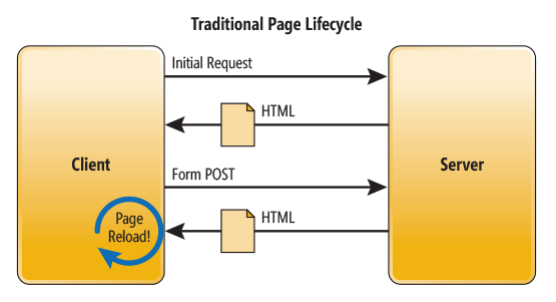
\includegraphics[width=\linewidth]{traditional_lifecycle}

% TODO Präsentations-Komponenten & welche andere art von komponenten???
% TODO was sind vor/nachteile von spa?

\section{SPA Overview}

\begin{itemize}
    \item Plain HTML/CSS/JS Code (no plugin)
    \item No page reloads
    \item Working back button
    \item Bookmarkable Links
    \item (limited) offline functionality
    \item Uses RESTful Services for data access
\end{itemize}
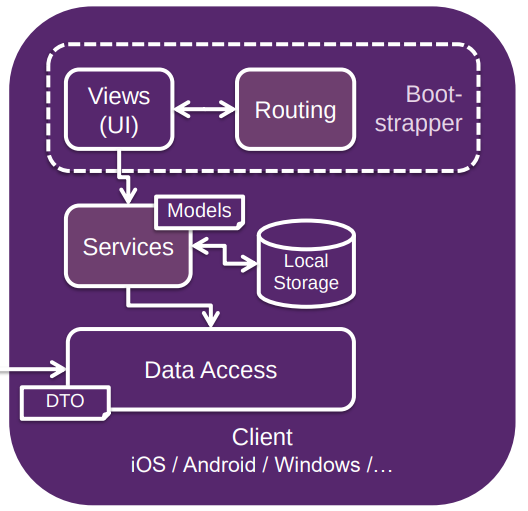
\includegraphics[width=.6\linewidth]{spa_arch}

\subsection{Routing}
Browser fakes the URL change.
\\
Use \textbf{Anchors \#} or \textbf{window.history} API

\subsection{Dependency Injection}
\begin{itemize}
    \item Reduced coupling between consumer and impl.
    \item Classes relate to each other not directly but by interfaces
    \item Allows flexible replacement of implementation
\end{itemize}

\subsection{Bundling with WebPack}
\begin{description}
    \item[Entry] Startpunkt wo Webpack mit Bundling beginnt und
    Dependencies findet.
    \item[Output] Where to bundle your application.
    \item[Loaders] Transformiert Dateien in Module. (\textit{module})
    \item[Mode] Enable built-in \textit{optimization} mechanisms.
\end{description}

\section{React}

Komponenten werden in Virtual DOM gerendert.

Virtual DOM Änderungen werden verglichen, erst dann werden wirkliche DOM Knoten erstellt.

\subsection{JSX}
JSX wird vom Präprozessor zu \mintinline{jsx}|React.createElement| Aufrufen umgewandelt => React import nötig!
\begin{minted}{jsx}
import React from 'react'

const menu = entries.map(entry =>
  <ListItem as="a" to={`/${entry.path}`}>
    <h1>{entry.title.toUpperCase()}</h1>
    <p className="lg">{entry.subtitle}</p>
  </ListItem>
);
\end{minted}

\subsubsection{Conditionals}
\begin{minted}{jsx}
{ error &&
    <Message>Fehler: {error}</Message> }
{ error ? <span>Fehler: {error}</span> : <span>OK!</span> }
\end{minted}

\subsubsection{Function \& Const}
\begin{minted}{jsx}
function HelloMessage(props) {
  return <div>Hi {props.name}</div>;
}
const HelloMessage = (props) => <div>Hi {props.name}</div>;
\end{minted}

\subsection{Mounting}
Komponenten müssen gemounted werden damit diese angezeigt werden können.
\begin{minted}{jsx}
const root = ReactDOM.createRoot(
  document.getElementById('root'));
root.render(<App />);
\end{minted}

\subsection{Props}
Alle Parameter sind in \textbf{props} Objekt. Read-only!

\subsection{State}
\begin{itemize}
    \item \textbf{useState} immer in derselben Reihenfolge aufrufen!
    \item Keine von Props abgeleiteten Daten im State!
    \item Props bevorzugen!
    \item Nur Dinge, die für GUI gebraucht werden in State
\end{itemize}

\begin{minted}{jsx}
const [value, setValue] = useState(0);
const increment = () => setCounter(counter + 1);
return <button onClick={increment}>Inc</button>
\end{minted}

\subsection{Formular}
\begin{minted}{jsx}
function handleSubmit(event) {
  // Damit Browser nicht Formular absendet
  event.preventDefault();
  alert(username + "," + password);//ajax
}
// ...
<button type="submit" onClick={handleSubmit}>Login</button>
\end{minted}

\subsection{Lifecycle}
Zusammengehörender Code auf mehrere Methoden verteilt:

\textit{Mount}: constructor -> render -> componentDidMount

\textit{Update}: render -> componentDidUpdate

\textit{Unmount}: componentWillUnmount

\begin{minted}{jsx}
useEffect(() => {
  const timerID = setInterval(
    () => setDate(new Date()), 1000);
  return () => { clearInterval(timerID) }
}, [])
\end{minted}

\subsection{Router}
\begin{minted}{jsx}
<BrowserRouter> // all routes inside tag
<Routes>
  <Route index element={<Home/>} />
  <Route path="/help" element ={<Help/>}/>
</Routes> // auch verschachtelung möglich
// don't use a tags now:
<Link to="/help">Help/Link>
\end{minted}

\subsection{Context}
\begin{minted}{jsx}
const ThemeContext = // param is default
  React.createContext(themes.light);
<ThemeContext.Provider value={themes.dark}>
</ThemeContext.Provider>
const theme = useContext(ThemeContext);
\end{minted}
\begin{itemize}
    \item ideal für globale read-only Props wie Themes
    \item Callbacks können auch durchgereicht werden
    \item Code wird bei vielen Context unübersichtlich
\end{itemize}

\subsection{Redux}
\begin{itemize}
    \item Action: \mintinline{javascript}|{ type: TRANSFER, amount: 100 }|
    \item Reducer erstellt neuen State-Tree mit Daten in Action
    \item Reducer sind pure Funktionen (no side effects)
    \item Reducer nur für Teil (Slice) von State-Tree zuständig
    \item Reducer werden zu Root Reducer kombiniert \mintinline{jsx}|combineReducers({balance, transactions})|
    \item Store wird mit Root Reducer erstellt \mintinline{jsx}|const store = createStore(rootReducer)|
    \item Einfachere Handhabung mit Redux Toolkit! (\mintinline{js}|createSlice({...})| Funktion, Immer library)
\end{itemize}

\subsubsection{Redux Toolkit}
\begin{minted}{js}
const balanceSlice = createSlice({
  name: "balance",
  initialState: { value: 0 },
  reducers: {
    transfer: (state, action) => {
      // "Immer" (Copy & Update Strategie)
      state.value += action.payload.amount;
    },
  },
});
export const {transfer} = balanceSlice.actions;
\end{minted}

\begin{itemize}
    \item Daten von API mit Redux Thunk laden (Middleware)
\end{itemize}

\subsubsection{Redux Vorteile/Nachteile}
\begin{itemize}
    \item Bessere Übersicht: State ist an einer Stelle
    \item Zustand kann serialisiert werden, ermöglicht Server Rendering
    \item Besseres Debugging da explizite Stateänderungen
    \item Einfachere React Komponenten!
    \item Hat \textbf{Overhead}! \(\Rightarrow\) Wenn kaum State existiert, der von mehreren Komponenten verwendet wird, lohnt sich Redux Overhead nicht
    \item Nicht jeder State muss ins Redux.\\Formulardaten/UI-State kann auch React State sein
\end{itemize}

\section{Angular}
für lang lebende \& komplexe Applikationen

\subsection{Modules}
\begin{minted}[breaklines]{ts}
@NgModule ({
  exports : [Type1, Type2, Module1] // The subset of declarations that should be visible and usable in the component templates of other modules.
  imports : [ CommonModule ], // Specifies modules from which exports / providers should be imported into this module.
  declarations : [] , // The view classes that belong to this module (components, directives and pipes ).
  providers : [] , // Creators of services that this module contributes to global collection of services (DI Container); they become accessible in all parts of app.
  bootstrap : [] // Main application view aka the root component. Only root module should set this property.
})
export class CoreModule { }
\end{minted}

\subsubsection{Group Exports}
Um zu vermeiden, dass exportierte Komponenten zweimal angegeben werden müssen!
\begin{minted}{ts}
const EXPORTED_DECLARATIONS: any[] = [Type1];
const INTERNAL_DECLARATIONS: any[] =
  [...EXPORTED_DECLARATIONS, Type2 ];
const EXPORTS: any[] = [...EXPORTED_DECLARATIONS, Module1];

declarations: INTERNAL_DECLARATIONS
exports: EXPORTS
\end{minted}

\subsubsection{Lazy Modules}
Make sure to not reference classes/components/... from Lazy Module from eagerly loaded application part. Otherwise it is already loaded!

\subsubsection{Module Types}
\begin{description}
    \item[Root/App] Provide entry point/bootstrap component for app. Imports BrowserModule. No exports.
    \item[Feature] Specify clear boundaries between application features. Allows to assign dev responsibilities to different teams.
    \item[Shared] Common components/directives/pipes and shares them with feature module. Don't specify app-wide singleton services here! (lazy-loaded module makes its own copy)
    \item[Core] Keeps Root Module clean. Contains components/directives/pipes used by Root Module. Globally used services can be declared here. Only Root Module should import this module.
\end{description}

\paragraph{Feature Module Sub Types}
\begin{description}
    \item[Domain] Deliver UI dedicated to particular app domain
    \item[Routing] Specifies routing specific configuration settings of Feature (or Root) module
    \item[Service] Provides utility services such as data access and messaging
    \item[Widget] Makes components/directive/pipes available to external modules
    \item[Lazy] Represents lazily loaded Feature Modules. (Routed Modules)
\end{description}

\subsection{Components}
\begin{itemize}
    \item Components allow to separate UI logic from representation
    \item Provide Information Hiding: Each Component declares a part of the UI
    \item \lstinline|selector| used to embed component into other view. (tag name (should be prefixed to avoid collisions!) or CSS-selector (\mintinline{css}|'#topHeader'|))
\end{itemize}

\begin{minted}{ts}
@Component({
  selector: 'wed-navigation',
  templateUrl: './navigation.component.html',
  styleUrls: ['./navigation.component.css']
})
export class NavigationComponent {}
\end{minted}

\subsubsection{Template Syntax}
\begin{itemize}
    \item Almost all valid HTML5 syntax is valid template syntax. But \mintinline{html}|<script>| is forbidden!
    \item HTML must be in valid format (\mintinline{html}|<p><h1></h1></p>| is not allowed)
    \item Operators with side effects/chaining are prohibited in "\mintinline{html+ng2}|{{}}|" Expressions (\mintinline{ts}|++ -- new = += , ...|)
\end{itemize}

\subsubsection{Binding}
\begin{description}
    \item[One-way in] Model to view \mintinline{html+ng2}|<p>{{counter.team}}</p>|, \\
      \mintinline{html+ng2}|<img [attr.alt]="counter.team" src="...">|
    \item[One-way call] View to Model (Event Binding) \\ \mintinline{html+ng2}|(click)="counter.eventHandler($event)"|
    \item[Two-way] \mintinline{html+ng2}|[(ngModel)]="counter.team"|
\end{description}

\subsubsection{Input and Output Properties}
\begin{description}
    \item[@Output()] component/directive fires bindable events
    \item[@Input()] component/directive consumes bindable values
\end{description}
\mintinline{html+ng2}|<wed-nav (click)=".." [title]=".."></wed->|
\begin{minted}{ts}
@Component({/*omitted*/})
export class NavigationComponent {
    @Output() click = new EventEmitter<any>();
    @Input() title: string;
}
\end{minted}

\subsubsection{Component Lifecycle}
ctor -> ngOnChanges -> ngOninit -> ngDoCheck -> ngOnDestroy

Do something in lifecycle: Implement hook methods. (interface e.g. \lstinline|OnInit| not needed but recommended)

\subsubsection{Content Projection (like props.children)}
Single-Slot: \mintinline{html+ng2}|<ng-content></ng-content>|

Multi-Slot:
\mintinline[breaklines]{html+ng2}|<ng-content select='menu'></ng-content>| \\
(or with tags: \mintinline{html+ng2}|select='[wed-title]'|)

\subsection{Directives}
\subsubsection{Attribute Directives}
\mintinline{html+ng2}|<div [ngClass]="hasWarning ? 'warn' : '' ">|
\subsubsection{Structural Directives}
\begin{itemize}
    \item Reshapes DOM structure (add, del, change elems)
\end{itemize}
\mintinline{html+ng2}|<div *ngIf="hasTitle"></div>|

\mintinline{html+ng2}|<li *ngFor="let element of elements"></li>|


\subsection{Template Reference Variables}
Reference DOM Element within template. Can also be reference to Angular component or directive.
\begin{minted}{html+ng2}
<input placeholder="phone number" #phone>
<button (click)="makeCall(phone.value)">Call</button>
\end{minted}

\subsection{Services}
\lstinline|@Injectable| marks class as an Injectable instance

\subsubsection{providedIn: root}
\begin{minted}{ts}
@Injectable({ providedIn: 'root' })
export class CounterService {}
\end{minted}
\mintinline{ts}|{providedIn: 'root'}| means service is registered for whole app. But this service is Tree-shakable.

\subsubsection{forRoot() / forChild()}
Create forRoot and forChild methods in module. In forRoot place service into providers. In forChild have no providers. forRoot should only be called from the AppModule / or CoreModule as it's only imported from AppModule.
\subsubsection{Async Services}
Use EventEmitter: \mintinline{ts}|this.xChanged.emit(this.x);|
\begin{minted}[breaklines]{ts}
// subscribe in ngOnInit and unsubscribe in ngOnDestroy
this.xService.xChanged.subscribe((x: XModel) => {this.x = x;});
\end{minted}

\subsection{Forms}
Template Driven and Reactive.

\subsubsection{Reactive Forms}
Form and Validation logic in Controller. Easier to test. Handles async validations. Designed for "daily" use.

\subsubsection{Template-driven Forms}
Less code but validation logic in HTML. More intuitive, simpler. Useful for small forms.

\begin{minted}[breaklines]{html+ng2}
<input type="text" id="name" required
  [(ngModel)]="model.name" name="name"
  #nameField="ngModel">
<div [hidden]="nameField.valid || nameField.pristine"
  >Name required</div>

<form (ngSubmit)="doLogin(sampleForm)" #sampleForm="ngForm">
  <button type="submit" [disabled]="!sampleForm.form.valid">Submit</button>
<form>
\end{minted}

\subsection{Angular Routing}
Define routes for a Module in their own RoutingModule.
Use RouterModule.\textbf{forRoot}(routes) only once on top level. Use \textbf{forChild}(routes) for sub-routing on all sub-levels.
\textbf{forRoot} contains all directive, given routes \textit{AND} singleton router service instance. \textbf{forChild} contains only directives, routes.

Use \mintinline{html+ng2}|<a routerLink="/home">| for links.

\mintinline{html+ng2}|<router-outlet>| defines where router should display views.
Can also be used in child.

\subsubsection{Route Configuration}
Router uses first-match-wins! More specific should be placed above less specific routes. Wildcard should abe last route! Use guards if route should only be activated in certain circumstances.

\textbf{pathMatch: 'full'} exact match.
\textbf{redirectTo: '/heroes'} redirect.
\textbf{path: '**'} wildcard.
\textbf{path: 'hero/:id'} maps e.g. /hero/42.

\subsection{Observables / HttpClient}
2 types with same API but different behavior:

\textbf{Hot Observables} for sequence of events, shared among all subscribers.
\textbf{Cold Observables} start running on subscribption (e.g. web requests), not shared among subscribers, automatically closed after task is finished

\textbf{Data Resource Services} should provide Observable interface.
\textbf{Business Layer Services} subscribe to the provided Observables. Allows caching, filtering, data aggregation and other business logic.

Intercept HTTP Requests with \textit{HttpInterceptor} for e.g. Authorization header.

\subsection{Streaming based business services}
It is possible to pull RxJS through all layers (Ui / Service / Data Resource). But in the end, this will result in async sections within the UI \(\Rightarrow\) Complex data management.

\subsection{Pipe Operator}
Pipes are good choice for small transformations. Can be chained.

\textbf{Custom Pipe}: Also add to declarations of module. Use @Pipe decorator.

async pipes make UI more complex.

\textbf{Predefined Pipes}: AsyncPipe, DecimalPipe, DatePipe, PercentPipe.

\textbf{No Filter / OrderBy pipe}. As these would need to be impure and therefore would perform very poorly. And they prevent aggressive minifcation. Do filtering/sorting inside controller.

\begin{minted}{html+ng2}
<p>{{counter.team | uppercase}}</p>
<p>{{counter.date | date:'longDate'}}</p>
\end{minted}

\begin{description}
    \item[Pure] By default. Only executed when Angular detects \textit{pure change} to input expression. Changes within composite objects/values are ignored.
    \item[Impure] Executed on \textit{every} component change detection cycle (every keystroke, mouse-move or other event). To reduce processing time caching is often seen inside impure pipes.
\end{description}

\subsection{Styling}
Selectors of SCSS file are local to that component! By default achieved with prepropressing. Native (Shadow DOM) implementation can be activated with changing encapsulation tag in @Component metadata.

\subsection{AOT}
Automatic when using production build. In Dev Build: uses JIT compiler by default which is delivered to client.

\section{ASP.NET}

\end{multicols*}
\end{document}